\documentclass{article}

% if you need to pass options to natbib, use, e.g.:
% \PassOptionsToPackage{numbers, compress}{natbib}
% before loading nips_2017
%
% to avoid loading the natbib package, add option nonatbib:
% \usepackage[nonatbib]{nips_2017}

\usepackage[final]{nips_2017}

% to compile a camera-ready version, add the [final] option, e.g.:
% \usepackage[final]{nips_2017}

%Pour langue et caractÚres spéciaux
\usepackage[french]{babel} 
\usepackage[T1]{fontenc}
%\usepackage{lmodern}
\usepackage[utf8]{inputenc}

%\usepackage[utf8]{inputenc} % allow utf-8 input
%\usepackage[T1]{fontenc}    % use 8-bit T1 fonts
\usepackage{hyperref}       % hyperlinks
\usepackage{url}            % simple URL typesetting
\usepackage{booktabs}       % professional-quality tables
\usepackage{amsfonts}       % blackboard math symbols
\usepackage{nicefrac}       % compact symbols for 1/2, etc.
\usepackage{microtype}      % microtypography
\usepackage{graphicx}
\usepackage{mathtools}
\usepackage{amsmath}


\title{Sur la classification d'étoiles en fonction de leur spectre d'absorption par apprentissage automatique}

% The \author macro works with any number of authors. There are two
% commands used to separate the names and addresses of multiple
% authors: \And and \AND.
%
% Using \And between authors leaves it to LaTeX to determine where to
% break the lines. Using \AND forces a line break at that point. So,
% if LaTeX puts 3 of 4 authors names on the first line, and the last
% on the second line, try using \AND instead of \And before the third
% author name.

\author{
  Patrice~B\'echard\\
  D\'epartement d'informatique\\
  et de recherche op\'erationelle\\
  Universit\'e de Montr\'eal\\
  Montr\'eal, QC H3T 1J4 \\
  \texttt{patrice.bechard@umontreal.ca} \\
  %% examples of more authors
  \And
  Jean-Pascal~Gu\'evin \\
  D\'epartement de math\'ematiques\\
  et de statistique \\
  Universit\'e de Montr\'eal\\
  Montr\'eal, QC H3T 1J4 \\
  \texttt{jean-pascal.guevin@umontreal.ca} \\
  %% \AND
  %% Coauthor \\
  %% Affiliation \\
  %% Address \\
  %% \texttt{email} \\
  %% \And
  %% Coauthor \\
  %% Affiliation \\
  %% Address \\
  %% \texttt{email} \\
  %% \And
  %% Coauthor \\
  %% Affiliation \\
  %% Address \\
  %% \texttt{email} \\
}

\begin{document}
% \nipsfinalcopy is no longer used

\maketitle
\vspace{-0.8cm}
\begin{center}
\textbf{IFT6390 - Fondements de l'apprentissage machine - \today}
\end{center}

\begin{abstract}
La classification de spectres stellaires provenant du \textit{Sloan Digital Sky Survey} a été effectuée par trois algorithmes d'apprentissage, soit les machines à vecteurs de support, les réseaux de neurones de type perceptron multicouche et les réseaux de neurones convolutifs. Un taux de classification $93.40\%$ a été obtenu avec les SVM, $94.41\%$ avec les MLP et $94.57\%$ avec les CNN. Une tâche similaire a été conduite avec des données d'électrocardiogramme avec des résultats moins concluants. Les taux de classification obtenus sont de $61.36\%$ pour les SVM, $60.69\%$ pour les MLP et $77.39\%$ pour les CNN.
\end{abstract}

% Introduction
\section{Introduction}

L'exploration de notre univers observable a amené les astrophysiciens à observer et à catégoriser des centaines de milliers d'étoiles en fonction notamment de leur taille, de leur masse, de leur température et de leur composition. Ce processus de classification se fait, entre autre, à partir du spectre d'absorption des étoiles qui est une mesure de l'intensité du spectre électromagnétique émis par celles-ci en fonction de la longueur d'onde. Une automatisation efficace de ce processus pourrait par conséquent être un grand avantage. Nous proposons donc trois algorithmes de classification d'étoiles en fonction de leur type spectral à l'aide de méthodes d'apprentissage automatique.  Pour la validation des algorithmes, des données d'électrocardiogramme, étant aussi des données corrélées en 1 dimension, seront utilisées. Les algorithmes d'apprentissage utilisés pour effectuer la classification sont les réseaux de neurones de type MLP, les réseaux de neurones convolutifs (CNN) ainsi que les machines à vecteur de support (SVM) à noyau souple. Les bases de données ainsi que les algorithmes d'apprentissages utilisés sont présentés en détails à la section \ref{sec:methods} et les résultats obtenus sont présentés à la section \ref{sec:results}. Les codes et les figures présentées pour l'ensemble du projet sont disponibles en ligne sur GitHub : \url{https://github.com/patricebechard/Machine_learning_IFT6390}.


% Presentation des algorithmes et bases de donnees
\section{Méthodes}\label{sec:methods}

Les données utilisées pour les spectres d'étoiles proviennent de la base de données \textit{Sloan Digital Sky Survey} (SDSS) \textit{Science Archive Server} (SAS) donnant gratuitement accÚs aux observations faites par différents télescopes. Il est évidemment nécessaire de traiter les spectres obtenus par le biais du SDSS, ceux-ci étant généralement trÚs bruités. Un processus lissage et de normalisation utilisant notamment des moyennes mobiles permet d'en extraire l'information pertinente en éliminant le plus possible le bruit et en ne conservant que ce qui semble correspondre à des tendances plus globales. De plus, chaque spectre a été tronqué de sorte que seul la section correspondant aux log-longueurs d'onde entre $3.65$ et $3.80$ -- correspondant aux longueurs d'onde entre $\approx 398.1$ nm jusqu'à $\approx 707.9$ nm, ce qui représente le spectre de lumiÚre visible -- a été conservé. Nous avons aplati les spectres en ajustant une courbe de degré 3 aux données et divisé par celle-ci. Finalement, une interpolation linéaire de points a permis de diminuer le nombre de traits caractéristiques à 1000, ce que les algorithmes peuvent manipuler sans problÚme. Un échantillon de 60000 étoiles réparti également pour 6 types spectral différents utilisés (A, F, G, K, M, WD) a été traité. Puisque ces spectres sont les seules entrées des algorithmes essayés, le prétraitement des données a un impact majeur sur les résultats. La figure \ref{fig:preprocessing_sdss} présente un exemple d'un spectre d'étoile avant et aprÚs avoir subi le processus de prétraitement. Ce processus est implémenté par le module \texttt{XXXXXXXXX} qui permet également d'extraire les données directement de SDSS.

\begin{figure}[!htb]
 \begin{minipage}{0.45\textwidth}
   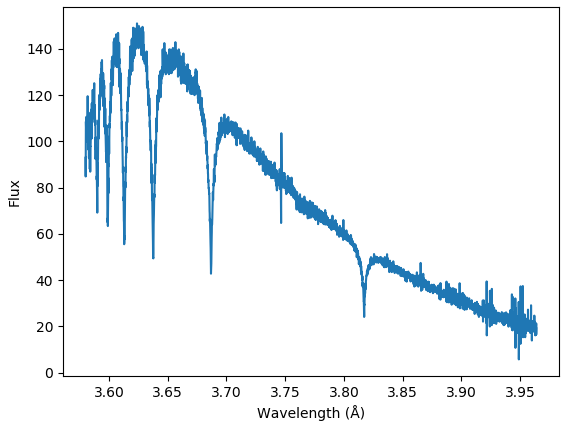
\includegraphics[width=\linewidth]{figures/sdss_raw.png}
 \end{minipage}\
 $\xRightarrow{\text{preprocessing}}$
 \begin{minipage}{0.45\textwidth}
   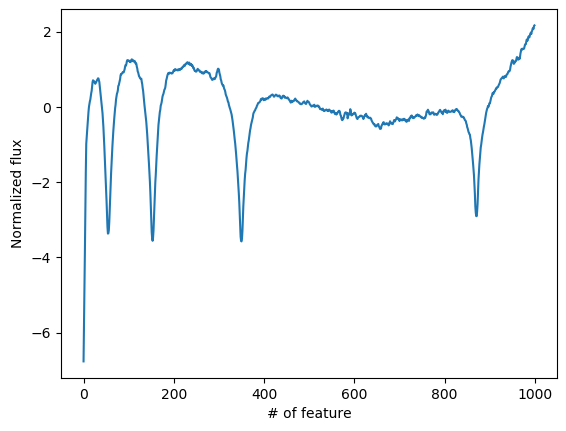
\includegraphics[width=\linewidth]{figures/sdss_norm.png}
 \end{minipage}\
 \caption{Effet du prétraitement des spectres d'étoiles. À gauche, un exemple de données brutes fournies par le \textit{Sloan Digital Sky Survey} est présenté. À droite, le même exemple a été normalisé et lissé.}\label{fig:preprocessing_sdss}
\end{figure}

Une premiÚre validation des algorithmes est effectuée par le biais d'une tâche connexe, soit la classification d'électrocardiogrammes selon l'état de santé du patient duquel il provient. Les électrocardiogrammes (ECG) étant fort semblables dans leurs formes à des spectres d'étoiles (tous deux étant des données corrélées dans l'espace en 1 dimension), ceci permet un premier ajustement des algorithmes en plus de nous initier au fonctionnement de ceux-ci dans le contexte d'une analyse spectroscopique. Les électrocardiogrammes utilisés proviennent du \textit{PhysioNet/Computing in Cardiology Challenge 2017} et ont l'avantage d'être plus simple à analyser, puisqu'ils sont plus lisses et moins bruités. Une séquence de 10 secondes a été conservée pour chaque ECG et les séquences ont été classées en 2 catégories, soit un patient en santé (5050 exemples), soit un patient avec une arythmie ou un autre problÚme cardiaque (3478 exemples). Le nombre de traits caractéristiques pour cet ensemble de données est de 500 pour chaque exemple. Le prétraitement des données est implémenté par le module \texttt{XXXXXXX}.

Trois familles d'algorithmes seront étudiées dans le cadre de ce projet. Tout d'abord, nous utiliserons des réseaux de neurones de type perceptron multicouche (MLP). L'usage de librairies telles Keras ou TensorFlow rend trÚs simple l'implémentation de ce type d'algorithme. Le réseau créé prendra en entrée un spectre traité (centré, réduit et lissé) et retournera en sortie la classification du spectre selon un encodage \textit{onehot}. La méthodologie utilisée pour ajuster les hyperparamÚtres (nombre de couches cachées, nombre de neurones dans chaque couche, régularisation, taille des lots) consiste à faire un \textit{grid search} sur plusieurs architectures de réseaux ainsi que plusieurs types de régularisation et plusieurs tailles de lots pour trouver une ou plusieurs combinaisons prometteuses en mesurant l'erreur de classification sur l'ensemble de validation. Un processus de \textit{fine tuning} des paramÚtres suivait ensuite pour améliorer le plus possible l'efficacité de l'algorithme. Finalement, un réentraînement sur l'ensemble d'entraînement ainsi que l'ensemble de validation avait lieu, accompagné d'un test sur l'ensemble de test nous a permis d'obtenir les résultats finaux. Une présentation en détails des résultats obtenus est faite à la section \ref{sec:results}. L'utilisation d'un processeur graphique (GPU) nous a permis d'effectuer une panoplie de différentes expériences sans que celles-ci soient trop coûteuses en temps. Des travaux similaires ont été menés par \cite{bailer1998automated} ainsi que \cite{carricajo2004automatic} pour les spectres stellaires, et par \cite{shensheng2017deep} pour les électrocardiogrammes.

Ensuite, puisque les points formant un spectre sont corrélés entre eux, les réseaux de neurones convolutifs (CNN) sont une approche d'apparence prometteuse. Le réseau créé calculera des convolutions unidimensionnelles sur les spectres. Le nombre de convolutions, de \textit{feature maps} ainsi que le type de \textit{pooling} (max, moyen, etc.) souhaités sont les hyperparamÚtres à déterminer. Ce type d'algorithme permet de réduire le nombre de dimensions du problÚme en plus de prendre en compte des caractéristiques des entrées comme la connectivité locale des traits caractéristiques, tout en introduisant une invariance des traductions locales grâce au \textit{pooling}. \cite{hala2014spectral} a mené des travaux similaires pour les spectres d'étoiles. Plusieurs travaux de recherche, notamment par \cite{rajpurkar2017cardiologist} ainsi que \cite{zihlmann2017convolutional} se sont penchés sur la classification d'électrocardiogrammes à l'aide de réseaux de neurones convolutifs.

Enfin, les machines à vecteur de support (SVM) à noyau souple seront le dernier type d'algorithme d'apprentissage utilisé pour la classification des spectres stellaires ainsi que des électrocardiogrammes. Ce genre d'algorithme a tendance à bien se débrouiller avec des entrées possédant un grand nombre de traits caractéristiques. Le noyau à utiliser sera déterminé lors de la sélection du modÚle. L'implémentation des SVM a été effectuée à l'aide de la librairie Scikit Learn. Des travaux similaires ont été menés par \cite{bu2014stellar} pour la classification de spectres d'étoile et par \cite{shensheng2017deep} pour les électrocardiogrammes.



% Resultats

\section{Présentation des résultats}\label{sec:results}

%%%%%%%%% ELECTROCARDIOGRAMMES
\subsection{Électrocardiogrammes}

Contrairement à ce à quoi nous nous attendions, nous avons eu beaucoup plus de problÚmes avec les données d'électrocardiogramme qu'avec les données de spectres stellaires. Tout d'abord, pour les SVM, des tests ont été effectués pour déterminer le noyau du SVM à utiliser parmi ceux implémentés par défaut dans Scikit Learn. Nous avons conservé le noyau mou de type polynomial (\texttt{poly}, $(\gamma\langle~x,~x'~\rangle~+~r)^d$) et un noyau à fonction à base radiale (\texttt{rbf}, ~$\exp(-\gamma||x-x'||_2 ^2)$). D'autres noyaux (linéaire, sigmoid) ont également été testés, mais le faible taux de succÚs obtenu les ont rapidement discrédités. L'effet de trois hyperparamÚtres a été étudié pour cet algorithme: le noyau utilisé, le degré du polynÎme dans le cas d'un noyau polynomial et la valeur de la constante de régularisation $C$ puisqu'il s'agit d'un \textit{soft kernel} SVM. La table~\ref{tab:ecg_preprocessing} montre les taux de classification obtenus pour ces hyperparamÚtres.

\begin{table*}[htb]
  \caption{Taux de classification obtenu avec l'algorithme SVM pour les trois noyaux étudiés.}
  \vspace{0.2cm}
  \label{tab:ecg_preprocessing}
  \centering
  \begin{tabular}{lllllll}
    \toprule
    & \multicolumn{3}{c}{\sc{Ens. d'entraînement}} & \multicolumn{3}{c}{\sc{Ens. de validation}}\\
    \sc{Noyau} & $C=0.75$ & $C=1.0$ & $C=1.25$ & $C=0.75$ & $C=1.0$ & $C=1.25$ \\
    \midrule
    RBF          & 74.42\% & 85.68\% & 91.24\% & 59.68\% & 60.24\% & 59.61\% \\
    Poly. deg. 2 & 85.29\% & 89.45\% & 91.73\% & 61.08\% & 61.37\% & 60.94\% \\
    Poly. deg. 3 & 93.39\% & 98.03\% & 98.84\% & 59.68\% & 58.13\% & 56.09\% \\
    \bottomrule
  \end{tabular}
\end{table*}

On note d'abord à quel point cet algorithme appliqué à cet ensemble de données est à risque de sur-apprentissage. En effet, pour chacun des noyaux, le taux classifications atteint $90\%$ et plus dÚs que $C\geq1$. Pourtant, pour des valeurs de $C$ à peine inférieure à 1, on est clairement en présence de sous-apprentissage, d'autant plus que les matrices de confusions montrent que tous les éléments sont classés dans la même catégorie. L'étroitesse de la fenêtre entre ces deux pÎles à éviter s'explique par la faible de taille de l'ensemble d'entraînement. Il apparaît évident que nous aurions davantage de latitude pour l'entraînement des paramÚtres si nous étions en possession d'un plus grand nombre de données. Des propositions permettant de contourner seront discutés à la section~\ref{sec:conclusion}. Il est aussi pertinent de se questionner sur la validité du prétraitement des données pour notre problÚme.

Une premiÚre tentative de diminuer le risque de sur-apprentissage est d'utiliser la technique d'analyse des composantes principales (PCA) afin de diminuer la dimension des traits caractéristiques, similairement à \cite{polat2007detection}. Les tables~\ref{tab:ecg_pca_300} et \ref{rab:ecg_pca_100} montrent les taux de classification obtenus lorsque les 300 et les 100 premiÚres composantes principales sont conservées. L'hypothÚse était qu'une diminution du nombre de traits caractéristiques diminuerait le nombre de paramÚtre du SVM également, ce qui devrait résulter en une baisse de la capacité du SVM. Le même phénomÚne que sans l'usage de PCA se produit cependant: on passe de sous-apprentissage à sur-apprentissage sans que le taux de classification de l'ensemble de validation n'augmente.

Une derniÚre tentative d'améliorer les résultats est d'appliquer aux données une transformée de Fourier. En effet, puisque les données représentent un signal, il pourrait être avantageux d'étudier les fréquences principales de ce signal plutÎt que le signal lui-même. Une démarche similaire a été conduite par \cite{gothwal2011cardiac} pour prétraiter les entrées d'un réseau de neurones. La figure ~\ref{fig:ecg_val_c} en annexe montre les taux de classification obtenus pour le noyau polynomial de degré 2 pour différentes valeurs de $C$. Le ta table \ref{tab:ecg_fourier} montre le taux de classification pour les différents noyaux. L'exact même phénomÚne se reproduit cependant: l'algorithme passe du sous-apprentissage au sur-apprentissage sans que l'erreur de classification de l'exemple de validation ne diminue. La figure~\ref{XXXXX} illustre cela: on y voit que le taux de bonnes classifications augmente pour l'ensemble d'entraînement, mais pas pour l'ensemble de validation.

On conclue que le meilleur classeur SVM à noyau \textit{soft} est celui envoyant tous les électrocardiogrammes à la même classe, ce qui est le cas pour le noyau polynomial de degré 2 et pour le noyau de type RBF pour $C=1$. C'est deux classeurs obtiennent des résultats d'environ $60\%$ sur l'ensemble test, ce qui est seulement dû à la répartition des électrocardiogrammes dans les classes sain et malade. Le résultat d'un tel classeur aurait été de $50\%$ si les répartitions avaient été égales. On conclue que le SVM s'applique mal à cet ensemble de données puisqu'il s'avÚre incapable de généraliser ses résultats. Notons que l'implémentation du SVM pour les données ECG est effectuée dans \texttt{XXXXXX}

Des résultats similaires ont été obtenus avec les réseaux de neurones de type MLP. Pour l'ensemble des réseaux de neurones de ce rapport, l'optimiseur \textit{Adam} a été utilisé, la fonction d'activation ReLU a été utilisée dans le réseau et la fonction softmax a été utilisée à la sortie. AprÚs un \textit{grid search} sur plusieurs architectures différentes, nous avons trouvé une architecture de réseau possédant deux couches cachées de 250 et 100 neurones, respectivement. Nous avons utilisé comme entrée des neurones les données prétraitées normalement (normalisées) ainsi que les données aprÚs y avoir effectuer une transformée de Fourier. Nous avons utilisé un terme de régularisation $\lambda$ de $0.0005$ pour une régularisation de type $L1$ et $L2$. La courbe d'apprentissage en fonction du nombre d'époques est présenté à la figure \ref{fig:ecg_dnn_train} en annexe. Comme on le voit, l'implémentation utilisant les données traitées par transformée de Fourier ont peine à dépasser $60\%$ de taux de classification, alors que celles utilisant les données normalisées atteignent à peine $58\%$, alors qu'il classe tous les exemples dans la même catégorie. Le module \texttt{XXXXX} implémente les réseaux de neurones pour les données ECG.

Finalement, en utilisant un CNN pour faire la détection d'arythmies cardiaques, nous avons essayé plusieurs configurations pour maximiser la classification. En mettant un CNN et un réseau MLP complÚtement connecté bout-à-bout, nous avons vérifié l'erreur de classification en faisant varier le nombre de couches de convolution et de pooling. Nous avons gardé le MLP constant d'expérience en expérience avec une couche cachée de 50 neurones. Nous nous sommes limités à des tailles de fenêtres de convolution de largeur 4 et des filtres de pooling de largeur 4. Nous n'avons pas jugé nécessaire de tester le CNN avec les données prétraitées à l'aide de PCA ou d'une transformation de Fourier. Le taux de classification sur l'ensemble de validation en fonction du nombre de convolutions est résumé au tableau \ref{tab:n_conv_ecg} en annexe. Notons que ces résultats correspondent au nombre optimal d'époques d'entraînement pour chaque combinaison d'hyperparamÚtres. Ceci sera également le cas pour tous les tableaux présentant des résultats des MLP et des CNN discutés dans cet article.


L'évolution de l'apprentissage en fonction du nombre d'époques d'entraînement pour le réseau convolutionnel avec 4 convolutions présenté au tableau \ref{tab:n_conv_ecg} testé sur l'ensemble de test est présenté à la figure \ref{fig:ecg_cnn_train}.

\begin{figure}[htbp]
\begin{center}
\includegraphics[width=0.6\textwidth]{figures/ecg_cnn_train.png}
\caption{Évolution du taux de classification sur les données d'électrocardiogramme en fonction du nombre d'époques d'entraînement pour le réseau de neurones convolutif avec 4 convolutions. }
\label{fig:ecg_cnn_train}
\end{center}
\end{figure}


Les résultats finaux de la précision de chaque algorithmes sur les électrocardiogrammes sont présentés au tableau \ref{tab:ecg_final_results}. Les résultats présentés sont ceux pour lesquels les meilleurs résultats ont été obtenus.

\begin{table*}[htb]
  \caption{Résultats pour la classification d'électrocardiogrammes sur l'ensemble de test pour chaque algorithme utilisé.}
  \vspace{0.2cm}
  \label{tab:ecg_final_results}
  \centering
  \begin{tabular}{llll}
    \toprule
    \sc{Algorithme}     & SVM     & MLP & CNN \\
    \midrule
    \sc{Précision} & 61.37\%  & 60.69\%   & 77.39\%  \\
    \bottomrule
  \end{tabular}
\end{table*}

Comme attendu, on remarque que le taux de classification des CNN est de plus de 16\% plus élevé que celui obtenu avec les autres algorithmes. Cette situation avait été anticipée, puisque les traits caractéristiques des signaux d'électrocardiogrammes sont autocorrélées. Le module \texttt{XXXXXX} implémente les CNN pour les données ECG.


%%%%%%%%%%%%%% SDSS


\subsection{Spectres d'étoiles}

Les résultats obtenus pour la classification de spectres stellaires ont été beaucoup plus concluants que ceux obtenus pour la classification d'électrocardiogrammes. Tout d'abord, avec les SVM, nous avons sélectionné un noyau RBF, puis avons essayé plusieurs valeurs pour la constante de pénalité $C$. Les résultats obtenus sont présentés à la figure \ref{fig:sdss_svm} en annexe. On voit que la constante $C$ a un effet important sur les résultats obtenus, et que la valeur optimale de $C$ s'avÚre être *********. Le module \texttt{XXXXXX} implémente le SVM pour les données de SDSS.

Pour les réseaux de neurones, nous avons essayé plusieurs architectures au hasard et avons aussi modifier la taille des lots et la régularisation pour l'apprentissage. Encore une fois, les non-linéarités choisies dans le réseau étaient de type {ReLU} et celles à la sortie étaient de type \textit{softmax}. La table \ref{fig:arch_sdss_dnn} en annexe présente le taux de classification obtenu pour différentes architectures de réseau de neurones. L'effet de l'architecture sur le taux d'apprentissage était minime, ne faisant varier celui-ci que par moins de 1\% à taille de lot constant (50) et sans régularisation. Les résultats de classification dépendent donc davantage du \textit{seed} que de ces hyperparamÚtres.

Le second hyperparamÚtre à ajuster pour régler la capacité du modÚle est la taille des lots. Pour le MLP avec les couches cachées $[150,100,50]$, plusieurs tailles de lots ont été testées et les résultats sont rapportés à la table \ref{tab:batch_sdss_dnn}. Encore une fois, le taux de classification ne varie que de trÚs peu pour différentes tailles de lots.  Finalement, nous avons essayé plusieurs types de régularisations pour le même réseau de neurones. La figure \ref{fig:reg_sdss_dnn} présente l'effet de la régularisation sur le taux de classification maximale. Les résultats obtenus grâce à la régularisation n'ont pas non plus eu beaucoup d'influence sur le taux de classification. Les réseaux de neurones sont implémentés pour les données de SDSS par le module \texttt{XXXXX}.

Enfin, un algorithme de type réseau de neurones convolutif à été étudié pour l'ensemble de données SDSS. Les hyperparamÚtres étudiés sont le nombre de convolution ainsi que le nombre de \textit{feature maps}, le \textit{batch size} et le nombre de couches cachées ainsi que le nombre de neurones les composant du réseau de neurones transmettant le vecteur de sortie du CNN à la sortie du réseau.Mentionnons également qu'un \textit{max pooling} est effectué aprÚs chaque convolution.

D'abord, le nombre de convolutions effectuées à été étudié pour des nombres variables de \textit{feature maps}. Pour ces essais, le réseau de neurone à la sortie du CNN a été gardé identique avec une couche cachée de taille 10 et fonctions d'activation ReLU et softmax. Les \textit{batch size} sont également demeurés constant à 50. La table~\ref{tab:sdss_cnn_conv} en annexe montre les taux de classifications obtenus pour l'ensemble de validation pour quelques unes de ces combinaisons. Les résultats obtenus sont relativement similaires, mais tentons d'optimiser les autres hyperparamÚtres pour la configuration [10, 50].

Essayons différents \textit{batch size} afin de pouvoir observer l'effet de cet hyperparamÚtre. La table~\ref{tab:sdss_cnn_bs} en annexe montre les résultats obtenus pour des \textit{batch size} de respectivement 5, 50 et 500. On voit que le choix des \textit{batch size} n'a que peu d'influence sur le taux de classification. Néanmoins, puisque ce sont des \textit{batch size} de 50 qui donnent de (légÚrement) meilleurs résultats, prenons cette valeur pour la suite des choses.

Enfin, optimisons la taille de la couche cachée du réseau de neurone en sortie du CNN. Les architectures considérées sont celles se trouvant à la table~\ref{tab:sdss_cnn_dnn} en annexe. Encore une fois, on voit qu'il n'y a que trÚs peu de différence entre les différentes valeurs de ces hyperparamÚtres. On note cependant que c'est une seule couche cachée de taille 50 qui a donné les meilleurs résultats.

Concluons cette analyse en notant que les hyperparamÚtres n'avaient pratiquement aucun effet sur les taux de classification obtenus. Cela signifie probablement que l'ensemble de données est en général trÚs facile à classer. On peut imaginer que les données forment des \textit{clusters} bien définis dans l'espace des traits caractéristiques sauf pour environ 5\% des spectres qui se mélangent à des \textit{clusters} d'une autre classe que la leur. Il est donc facile d'obtenir environ 94\% de bonnes classifications sur un ensemble test, mais il serait trÚs ardu d'obtenir davantage. On remarque également que le taux classification pour l'ensemble d'entraînement, bien que plus élevé que celui de l'ensemble de validation, n'a jamais atteint 100\%, ce qui est cohérent avec l'hypothÚse proposée. Le module \texttt{XXXXX} implémente les CNN pour les données de SDSS.







Les résultats finaux de la précision de chaque algorithme sur les spectres stellaires sont présentés au tableau \ref{tab:sdss_final_results}.
\begin{table*}[htb]
  \caption{Résultats pour la classification de spectres d'étoiles pour chaque algorithme utilisé.}
  \vspace{0.2cm}
  \label{tab:sdss_final_results}
  \centering
  \begin{tabular}{llll}
    \toprule
    \sc{Algorithme}     & SVM     & MLP & CNN \\
    \midrule
    \sc{Précision} & \%  & \%   & 77.17\%  \\
    \bottomrule
  \end{tabular}
\end{table*}

% Discussion et conclusion
\section{Conclusion}\label{sec:conclusion}

\section{Répartition et remerciements}


\small
\bibliographystyle{apalike}
\bibliography{report}

\clearpage
\section*{Annexe}

%svm ecg

\begin{table*}[htb]
  \caption{Taux de classification obtenu avec l'algorithme SVM pour les trois noyaux étudiés avec utilisation du PCA avec les 300 premiÚres composantes principales conservées dans le prétraitement des données pour l'ensemble de données d'électrocardiogrammes.}
  \vspace{0.2cm}
  \label{tab:ecg_pca_300}
  \centering
  \begin{tabular}{lllllll}
    \toprule
     & \multicolumn{3}{c}{\sc{Ens. d'entraînement}} & \multicolumn{3}{c}{\sc{Ens. de validation}}\\
    \sc{Noyau} & $C=0.75$ & $C=1.0$ & $C=1.25$ & $C=0.75$ & $C=1.0$ & $C=1.25$ \\
    \midrule
    RBF          & 86.51\% & 95.62\% & 98.03\% & 58.97\% & 58.55\% & 58.48\% \\
    Poly. deg. 2 & 93.56\% & 95.34\% & 96.13\% & 53.91\% & 53.48\% & 53.55\% \\
    Poly. deg. 3 & 99.70\% & 99.88\% & 99.89\% & 55.03\% & 55.17\% & 54.54\% \\
    \bottomrule
  \end{tabular}
\end{table*}

\begin{table*}[htb]
  \caption{Taux de classification obtenu avec l'algorithme SVM pour les trois noyaux étudiés avec utilisation du PCA avec les 100 premiÚres composantes principales conservées dans le prétraitement des données pour l'ensemble de données d'électrocardiogrammes.}
  \vspace{0.2cm}
  \label{tab:ecg_pca_100}
  \centering
  \begin{tabular}{lllllll}
    \toprule
     & \multicolumn{3}{c}{\sc{Ens. d'entraînement}} & \multicolumn{3}{c}{\sc{Ens. de validation}}\\
    \sc{Noyau} & $C=0.75$ & $C=1.0$ & $C=1.25$ & $C=0.75$ & $C=1.0$ & $C=1.25$ \\
    \midrule
    RBF          & 97.98\% & 99.63\% & 99.86\% & 59.11\% & 58.34\% & 58.90\% \\
    Poly. deg. 2 & 91.05\% & 92.42\% & 93.77\% & 52.99\% & 53.41\% & 53.55\% \\
    Poly. deg. 3 & 99.98\% & 99.98\% & 99.98\% & 52.15\% & 52.01\% & 51.58\% \\
    \bottomrule
  \end{tabular}
\end{table*}

\begin{figure}[htbp]
\begin{center}
\includegraphics[width=0.8\textwidth]{figures/ecg_constant.png}
\caption{Évolution du taux de classification sur les données d'électrocardiogramme en fonction de la constante de pénalité C pour l'algorithme SVM avec des données transformées à l'aide d'une transformée de Fourier. }
\label{fig:ecg_val_c}
\end{center}
\end{figure}


\begin{table*}[htb]
  \caption{Taux de classification obtenu avec l'algorithme SVM pour les trois noyaux étudiés avec l'utilisation d'une transformée de Fourier lors du prétraitment des données pour l'ensemble de données d'électrocardiogrammes.}
  \vspace{0.2cm}
  \label{tab:ecg_fourrier}
  \centering
  \begin{tabular}{lllllll}
    \toprule
     & \multicolumn{3}{c}{\sc{Ens. d'entraînement}} & \multicolumn{3}{c}{\sc{Ens. de validation}}\\
    \sc{Noyau} & $C=0.5$ & $C=1.0$ & $C=1.5$ & $C=0.5$ & $C=1.0$ & $C=1.5$ \\
    \midrule
    RBF          & 59.54\% & 100.00\% & 100.00\% & 58.90\% & 58.90\% & 58.90\% \\
    Poly. deg. 2 & 100.00\% & 100.00\% & 100.00\% & 55.52\% & 55.52\% & 55.52\% \\
    Poly. deg. 3 & 100.00\% & 100.00\% & 100.00\% & 59.68\% & 54.40\% & 54.40\% \\
    \bottomrule
  \end{tabular}
\end{table*}

% dnn ecg

\begin{figure}[htbp]
\begin{center}
\includegraphics[width=0.8\textwidth]{figures/ecg_dnn_train.png}
\caption{Évolution du taux de classification sur les données d'électrocardiogramme en fonction du nombre d'époques d'entraînement pour le réseau de neurones de type MLP avec deux couches cachées de 250 et 100 neurones, respectivement. }
\label{fig:ecg_dnn_train}
\end{center}
\end{figure}

% cnn ecg

\begin{table*}[htb]
  \caption{Taux de classification en fonction du nombre de convolutions dans le réseau de neurones convolutionnel pour les données d'électrocardiogramme.}
  \vspace{0.2cm}
  \label{tab:n_conv_ecg}
  \centering
  \begin{tabular}{lll}
    \toprule
    \sc{Config.} & \sc{Ens. d'entraînement} & \sc{Ens. de validation} \\
    \midrule
    $[100]$          & 0.7962 & 0.6882 \\
    $[50, 100]$      & 0.7917 & 0.7476 \\
    $[10, 50, 100]$     & 0.7922 & 0.7672\\
    $[10, 50, 100, 200]$ & 0.8198 & 0.7792 \\
    \bottomrule
  \end{tabular}
\end{table*}



%svm sdss



%mlp sdss

\begin{table*}[htb]
  \caption{Taux de classification obtenu avec l'algorithme DNN pour l'ensemble de données SDSS pour différentes architectures.}
  \vspace{0.2cm}
  \label{tab:sdss_cnn_dnn}
  \centering
  \begin{tabular}{lll}
    \toprule
    \sc{Config.} & \sc{Ens. d'entraînement} & \sc{Ens. de validation} \\
    \midrule
    $[50]$           & 0.9732 & 0.9393 \\
    $[100]$          & 0.9774 & 0.9389 \\
    $[200]$          & 0.9553 & 0.9393 \\
    $[400]$          & 0.9778 & 0.9396 \\
    $[200, 100]$     & 0.9783 & 0.9439 \\
    $[200, 50]$      & 0.9715 & 0.9437 \\
    $[500, 100]$     & 0.9791 & 0.9436 \\
    $[150, 100, 50]$ & 0.9792 & 0.9456 \\
    $[500, 100, 50]$ & 0.9812 & 0.9431 \\
    \bottomrule
  \end{tabular}
\end{table*}

\begin{table*}[htb]
  \caption{Taux de classification obtenu avec l'algorithme DNN pour l'ensemble de données SDSS en fonction \textit{batch size} pour l'architecture [150, 100, 50].}
  \vspace{0.2cm}
  \label{tab:sdss_cnn_dnn}
  \centering
  \begin{tabular}{lll}
    \toprule
    \sc{Batch size} & \sc{Ens. d'entraînement} & \sc{Ens. de validation} \\
    \midrule
    5           & 0.9684 & 0.9431 \\
    50          & 0.9729 & 0.9408 \\
    500         & 0.9794 & 0.9441 \\
    \bottomrule
  \end{tabular}
\end{table*}

%cnn sdss

\begin{table*}[htb]
  \caption{Taux de classification obtenu avec l'algorithme CNN pour l'ensemble de données SDSS en fonction du nombre de filtres de convolution par couche de convolution.}
  \vspace{0.2cm}
  \label{tab:sdss_cnn_conv}
  \centering
  \begin{tabular}{lll}
    \toprule
    \sc{Config.} & \sc{Ens. d'entraînement} & \sc{Ens. de validation} \\
    \midrule
    $[10]$          & 0.9741 & 0.9375 \\
    $[50]$          & 0.9902 & 0.9423 \\
    $[100]$         & 0.9862 & 0.9447 \\
    $[10, 50]$      & 0.9600 & 0.9457 \\
    $[50, 100]$     & 0.9896 & 0.9440 \\
    $[10, 50, 100]$ & 0.9741 & 0.9455 \\
    \bottomrule
  \end{tabular}
\end{table*}

\begin{table*}[htb]
  \caption{Taux de classification obtenu avec l'algorithme CNN pour l'ensemble de données SDSS en fonction de la taille des lots.}
  \vspace{0.2cm}
  \label{tab:sdss_cnn_bs}
  \centering
  \begin{tabular}{lll}
    \toprule
    \sc{Batch size} & \sc{Ens. d'entraînement} & \sc{Ens. de validation} \\
    \midrule
    5     & 0.9475 & 0.9413 \\
    50    & 0.9442 & 0.9440 \\
    500   & 0.9577 & 0.9431 \\
    \bottomrule
  \end{tabular}
\end{table*}

\begin{table*}[htb]
  \caption{Taux de classification obtenu avec l'algorithme CNN pour l'ensemble de données SDSS en fonction de l'architecture du réseau à la sortie du CNN.}
  \vspace{0.2cm}
  \label{tab:sdss_cnn_dnn}
  \centering
  \begin{tabular}{lll}
    \toprule
    \sc{Config.} & \sc{Ens. d'entraînement} & \sc{Ens. de validation} \\
    \midrule
    $[20]$          & 0.9591 & 0.9425 \\
    $[50]$          & 0.9626 & 0.9436 \\
    $[100]$         & 0.9802 & 0.9427 \\
    $[20, 50]$      & 0.9579 & 0.9404 \\
    $[50, 100]$     & 0.9768 & 0.9429 \\
    $[20, 50, 100]$ & 0.9435 & 0.9407 \\
    \bottomrule
  \end{tabular}
\end{table*}


\end{document}